\section{Case Studies} \label{sec:sc-usecases}

In this section, we provide three case studies demonstrating the practical
utility of cipher switching. We cover a wide range of situations, highlighting
concerns like meeting latency goals (\cref{subsec:uc3}), trading off security
and writable space (\cref{subsec:uc2}), and keeping within an energy budget
(\cref{subsec:uc1}). We also demonstrate the utility of both temporal and
spatial switching strategies, exploring the range of conditions under which
certain strategies are optimal.

\subsection{Balancing Security Goals with a Hard Energy Cap} \label{subsec:uc1}

Here we revisit the motivating example from \secref{sc-motivation}. It illustrates
that, because latency and energy use are correlated among the ciphers we
examined, we can exploit that to save battery life when necessary while
maintaining confidentiality when uploading encrypted backups to our
enterprise solution.

To simulate I/O activity, we begin randomly writing 10 40MB files using the
Freestyle Balanced cipher configuration over the course of approximately 120-125
seconds. After 5 seconds, the device enters ``battery saver'' mode, also pausing
backup uploads. We simulate this event by 1) underclocking the cores to their
lowest frequencies and 2) using \texttt{taskset} to transition the SwitchCrypt
processes to the energy-efficient LITTLE cores. After this event, we complete
the remaining workload using the ChaCha8 cipher. We repeat this experiment three
times.

\begin{figure}[ht] \textbf{Battery Saver Use Case: Energy-Security Tradeoff vs
   Strict Energy Budget}\par\medskip
   \centering
   {\begin{tikzpicture}[baseline]

    \pgfmathsetmacro{\xmax}{130} % set the maximum x value
    \pgfmathsetmacro{\ymax}{50} % set the maximum y value
    \pgfmathsetmacro{\ymaxbreak}{50.1} % set the y value at which overflow is drawn

    \begin{groupplot}[
        group style={
            group size=1 by 2,
            ylabels at=edge left,
            xlabels at=edge bottom,
            yticklabels at=edge left,
            xticklabels at=edge bottom,
            vertical sep=10pt,
        },
        %axis x line*=bottom,
        height=4cm,
        width=\linewidth,
        tick align=outside,
        tick pos=bottom, % make sure ticks only appear at the bottom and left axes
        tick style={ black },
        y tick label style={ /pgf/number format/fixed, /pgf/number format/precision=0 },
        grid style={ dotted, gray },
        every node near coord/.append style={font=\tiny},
        %
        % % magic to make the numbers appear above the overly long bars:
        % visualization depends on={rawy \as \rawy}, % save original y values
        % restrict y to domain*={ % now clip/restrict any y value to ymax
        %     \pgfkeysvalueof{/pgfplots/ymin}:\ymaxbreak
        % },
        % after end axis/.code={ % draw squiggly line indicating break
        %     \draw [semithick, white, decoration={snake,amplitude=0.1mm,segment length=0.75mm,post length=0.375mm}, decorate] (rel axis cs:0,1.01) -- (rel axis cs:1,1.01);
        % },
        % nodes near coords={\color{.!75!black}\pgfmathprintnumber\rawy}, % print the original y values (darkened in case they are too light)...
        % nodes near coords greater equal only=\ymax, % ... but ONLY if they are >= ymax
        clip=true, % allow clip to protrude beyond ymax if false
        % % Custom stuff to edit per template
        %
        xlabel={Time (s)},
        xlabel near ticks,
        xlabel shift={-4mm},
        xmin=0, xmax=\xmax,
        xtick={ 0, \xmax },
        enlargelimits=false, % add some breathing room along the x axis's sides
        % %major x tick style=transparent,
        %
        ylabel near ticks,
        ylabel shift={-2.5mm},
        ymajorgrids=true,
        %yticklabels={ 0, 0.5, 1.5, 2 },
        % extra y ticks={1},
        % extra y tick style={grid=major, grid style={dashed, black}},
        % extra y tick label={\empty},
        %bar width=4.5pt, % change size of bars
        %
        legend cell align=center,
        legend style={ column sep=1ex },
        legend entries={
            {\scriptsize Freestyle Balanced},
            {\scriptsize Freestyle Balanced + ChaCha8},
            {\scriptsize ChaCha8},
        },
        legend style={
            draw=none,
            legend columns=2,
            at={(0.5, 1.02)},
            anchor=south,
        },
    ]
        \nextgroupplot[ylabel={Energy Used (j)}, ymin=0, ymax=\ymax, ytick={ 0, \ymax }]
            \addplot [thick] table [
                x=time,
                y=energy,
                discard if symbol not={cipher}{fb},
                discard if symbol not={iop}{w},
                col sep=space,
                mark=none
            ] {data/sc/usecase-battery.dat};
            \addplot [thick, dashdotted] table [
                x=time,
                y=energy,
                discard if symbol not={cipher}{fb+c8},
                discard if symbol not={iop}{w},
                col sep=space,
                mark=none
            ] {data/sc/usecase-battery.dat};
            \addplot [thick, densely dashed] table [
                x=time,
                y=energy,
                discard if symbol not={cipher}{c8},
                discard if symbol not={iop}{w},
                col sep=space,
                mark=none
            ] {data/sc/usecase-battery.dat};
            \coordinate (c1) at (35, 16.5);
            \coordinate (c2) at (104, 45);
            \coordinate (c3) at (5, 45);
            \draw [dotted] (0, 34) -- (130, 34) node [above of=c1] {\tiny (energy ceiling)};
            \draw [dotted] (120, 0) -- (120, 50) node [right of=c2] {\tiny (battery dies)};
            \draw [dotted] (5, 0) -- (5, 50) node [right of=c3] {\tiny (battery critical)};
        \nextgroupplot[legend to name={throwaway7}, ylabel={R+R (norm)}, ymin=0, ymax=3, ytick={ 0, 0.5, 2.5, 3 }, yticklabels={ , 0, 1, }, ylabel shift={-1.5mm}]
            \addplot [thick] table [
                x=time,
                y=score,
                discard if symbol not={cipher}{fb},
                discard if symbol not={iop}{w},
                col sep=space
            ] {data/sc/usecase-battery.dat};
            \addplot [thick, dashdotted] table [
                x=time,
                y=score,
                discard if symbol not={cipher}{fb+c8},
                discard if symbol not={iop}{w},
                col sep=space
            ] {data/sc/usecase-battery.dat};
            \addplot [thick, densely dashed] table [
                x=time,
                y=score,
                discard if symbol not={cipher}{c8},
                discard if symbol not={iop}{w},
                col sep=space
            ] {data/sc/usecase-battery.dat};
            \draw [dotted] (0.585cm, 0) -- (0.585cm, 3.2cm);
            \draw [dotted] (13.80cm, 0) -- (13.80cm, 3.2cm);
    \end{groupplot}%
\end{tikzpicture}%
} \caption{Median sequential write total
   energy use with respect to time with respect to time.}
  \label{fig:usecase-battery}
\end{figure}

In \figref{usecase-battery}, we see time versus energy used. At 0 seconds, we
begin writing. At 5 seconds, the ``battery saver'' event occurs, causing the
system to be underclocked. At 120 seconds, the system will die. If we blow past
our energy ceiling, the system will die.

Our goal is to complete I/O before the device dies. We have three cipher
configuration choices. 1) Favor security even when backups are paused and use
Freestyle Balanced exclusively. Our results show that the device will die before
I/O completes. 2) Favor low energy use even when backups are being uploaded and
use ChaCha8 exclusively. Our results show that the device will finish writing
early, but we cannot safely upload backups when nuggets are encrypted using
ChaCha8. Finally, we have 3) favor security and use Freestyle Balanced when
uploading backups, and switch to ChaCha8 when the system enters the low power
state. Our results show that, while the system uses slightly more power in the
short term, we stay within our energy budget and finish before the devices dies.
Further, when we get our device to a charger, SwitchCrypt can converge nuggets
back to Freestyle Balanced and resume uploading backups.

On average, using Forward cipher switching resulted in a 3.3x total energy use
reduction compared to exclusively using Freestyle Balanced, allowing us to
remain within our energy budget. We note, however, that the energy savings is
not the point of this experiment. Rather, the lesson learned is that SwitchCrypt
enables the system to move to the right point in the energy/security tradeoff
space so that the current task can still be accomplished before the battery is
drained and without compromising backup security at any point.

\subsection{Variable Security Regions} \label{subsec:uc2}

This usecase illustrates utility of spatial Selective switching to achieve a
performance win over prior work where the entire drive is encrypted with a
single cipher. We demonstrate \emph{Variable Security Regions} (VSR), where we
can choose to encrypt select files or portions of files with different keys and
ciphers below the filesystem level.

Storing classified materials, corporate secrets, etc. require the highest level
of discretion, yet sensitive information like this can appear within a (much)
larger amount of data that we value less. But if only a small percentage of the
data needs the strongest encryption, then only a small percentage of the data
should have that associated overhead. In this scenario, a user wants to indicate
one or more regions of a file are more sensitive than the others. For example,
perhaps banking transaction information is littered throughout a PDF; perhaps
passwords and other sensitive information exists within several much larger
files. Using prior techniques, either all the data would be stored with high
overhead, the critical data would be stored without the mandated cipher type, or
the data would have to be split among separate files requiring potentially
complex and error-prone management schemes. SwitchCrypt VSRs allows us to
sidestep these issues.

We begin by with 10 5MB and 4KB write-read operations to two
SwitchCrypt instances: one using ChaCha8 (C8) and the other using Freestyle
Strong (FS). These results represent I/O without cipher switching where 100\% of
the data is stored with either high overhead (FS) or using an inappropriate
cipher (C8). We then use a third SwitchCrypt instance initialized with Selective
switching and write-read with a 7:3 ratio of ChaCha8 versus Freestyle
Balanced I/O operations. Here, 30\% of the data is considered sensitive. We
repeat this experiment three times.

\begin{figure}[ht] \textbf{VSR Use Case: ChaCha8 vs Freestyle Strong Sequential
4KB, 5MB Performance}\par\medskip
   \centering
   {\begin{tikzpicture}[baseline]

    \pgfmathsetmacro{\ymax}{20} % set the maximum y value
    \pgfmathsetmacro{\ymaxbreak}{20.1} % set the y value at which overflow is drawn

    \begin{axis}[
        %axis x line*=bottom,
        height=4cm,
        width=\linewidth,
        tick align=outside,
        tick pos=bottom, % make sure ticks only appear at the bottom and left axes
        tick style={ black },
        y tick label style={ /pgf/number format/fixed, /pgf/number format/precision=0 },
        grid style={ dotted, gray },
        every node near coord/.append style={font=\tiny},
        %
        % magic to make the numbers appear above the overly long bars:
        visualization depends on={rawy \as \rawy}, % save original y values
        restrict y to domain*={ % now clip/restrict any y value to ymax
            \pgfkeysvalueof{/pgfplots/ymin}:\ymaxbreak
        },
        after end axis/.code={ % draw squiggly line indicating break
            \draw [semithick, white, decoration={snake,amplitude=0.1mm,segment length=0.75mm,post length=0.375mm}, decorate] (rel axis cs:0,1.01) -- (rel axis cs:1,1.01);
        },
        nodes near coords={\color{.!75!black}\pgfmathprintnumber\rawy}, % print the original y values (darkened in case they are too light)...
        nodes near coords greater equal only=\ymax, % ... but ONLY if they are >= ymax
        clip=false, % allow clip to protrude beyond ymax
        % Custom stuff to edit per template
        %
        xlabel={\footnotesize Cipher Configuration},
        xlabel near ticks,
        xmin=C8, xmax=FS,
        xtick=data,
        symbolic x coords={C8,C8+FS,FS},
        enlarge x limits=0.2, % add some breathing room along the x axis's sides
        %major x tick style=transparent,
        %
        ylabel={\footnotesize Latency (s)},
        ylabel near ticks,
        ylabel shift={-1mm},
        ymajorgrids=true,
        ymin=0, ymax=\ymax,
        ybar, % value will shift bars
        ytick={ 0, 5, ..., \ymax },
        %yticklabels={ 0, 0.5, 1.5, 2 },
        % extra y ticks={1},
        % extra y tick style={grid=major, grid style={dashed, black}},
        % extra y tick label={\empty},
        %bar width=4.5pt, % change size of bars
        %
        legend cell align=center,
        legend style={ column sep=1ex },
        legend entries={
            {\scriptsize 4K/reads},
            {\scriptsize 4K/writes},
            {\scriptsize 5M/reads},
            {\scriptsize 5M/writes},
        },
        legend style={
            draw=none,
            legend columns=2,
            at={(0.5,1.02)},
            anchor=south,
        },
    ]
        \addplot[fill=orangeDark, every node near coord/.append style={color=orangeDark}]
        table[x=conf, y=latr-4k, col sep=space] {charts/usecase-vsr-tradeoff.dat};
        \addplot[fill=orangeDark, postaction={pattern=north east lines}, every node near coord/.append style={color=purpleDark}]
        table[x=conf, y=latw-4k, col sep=space] {charts/usecase-vsr-tradeoff.dat};
        \addplot[fill=purpleDark, every node near coord/.append style={color=orangeDark}]
        table[x=conf, y=latr-5m, col sep=space] {charts/usecase-vsr-tradeoff.dat};
        \addplot[fill=purpleDark, postaction={pattern=north east lines}, every node near coord/.append style={color=purpleDark}]
        table[x=conf, y=latw-5m, col sep=space] {charts/usecase-vsr-tradeoff.dat};
    \end{axis}%
\end{tikzpicture}%
} \caption{Median sequential read and write
   performance comparison of 4KB, 5MB I/O with 7-to-3 ratio, ChaCha8 vs
   Freestyle Strong (respectively).}
  \label{fig:usecase-vsr-bar}
\end{figure}

In \figref{usecase-vsr-bar}, we see the sequential read and write performance of
4KB and 5MB workloads when nuggets are encrypted exclusively with ChaCha8 or
Freestyle Balanced. Between them, we see Selective switching 7:3 ratio I/O
results.

Our goal is to use VSRs to keep our sensitive data at the mandated security
level while keeping the performance and battery life benefits of using a fast
cipher for the majority of I/O operations. Using SwitchCrypt Selective switching
versus prior work results in a reduction of 3.1x to 4.8x for read latency and
1.6x to 2.8x for write latency, all without compromising the security needs of
the most sensitive data.

\subsection{Responding to End-of-Life Slowdown in SSDs} \label{subsec:uc3}

This usecase illustrates using temporal Forward switching to offset the
debilitating decline in performance when SSDs reach end-of-life
(EoL)~\cite{SSDEOL1}. We demonstrate the utility of such a system to dynamically
stay within a strict latency budget while meeting minimum security requirements,
which is not possible using prior work.

Due to garbage collection and wear-leveling requirements of SSDs, as free space
becomes constrained, I/O performance drops precipitously~\cite{SSDEOL1}. With
prior work, our strict latency ceiling is violated. However, if SwitchCrypt is
made aware when the drive is in such a state, we can offset some of the
performance loss by switching the ciphers of high traffic nuggets to the fastest
acceptable cipher available using Forward switching.

We begin by writing 10 40MB files to SwitchCrypt per each cipher as a baseline.
We then introduce a delay into SwitchCrypt I/O of $20ms$, simulating drive
slowdown, and repeat the experiment three times.

\begin{figure}[ht] \textbf{SSD EoL Use Case: Latency-Security Tradeoff vs
   Goals}\par\medskip
   \centering
   {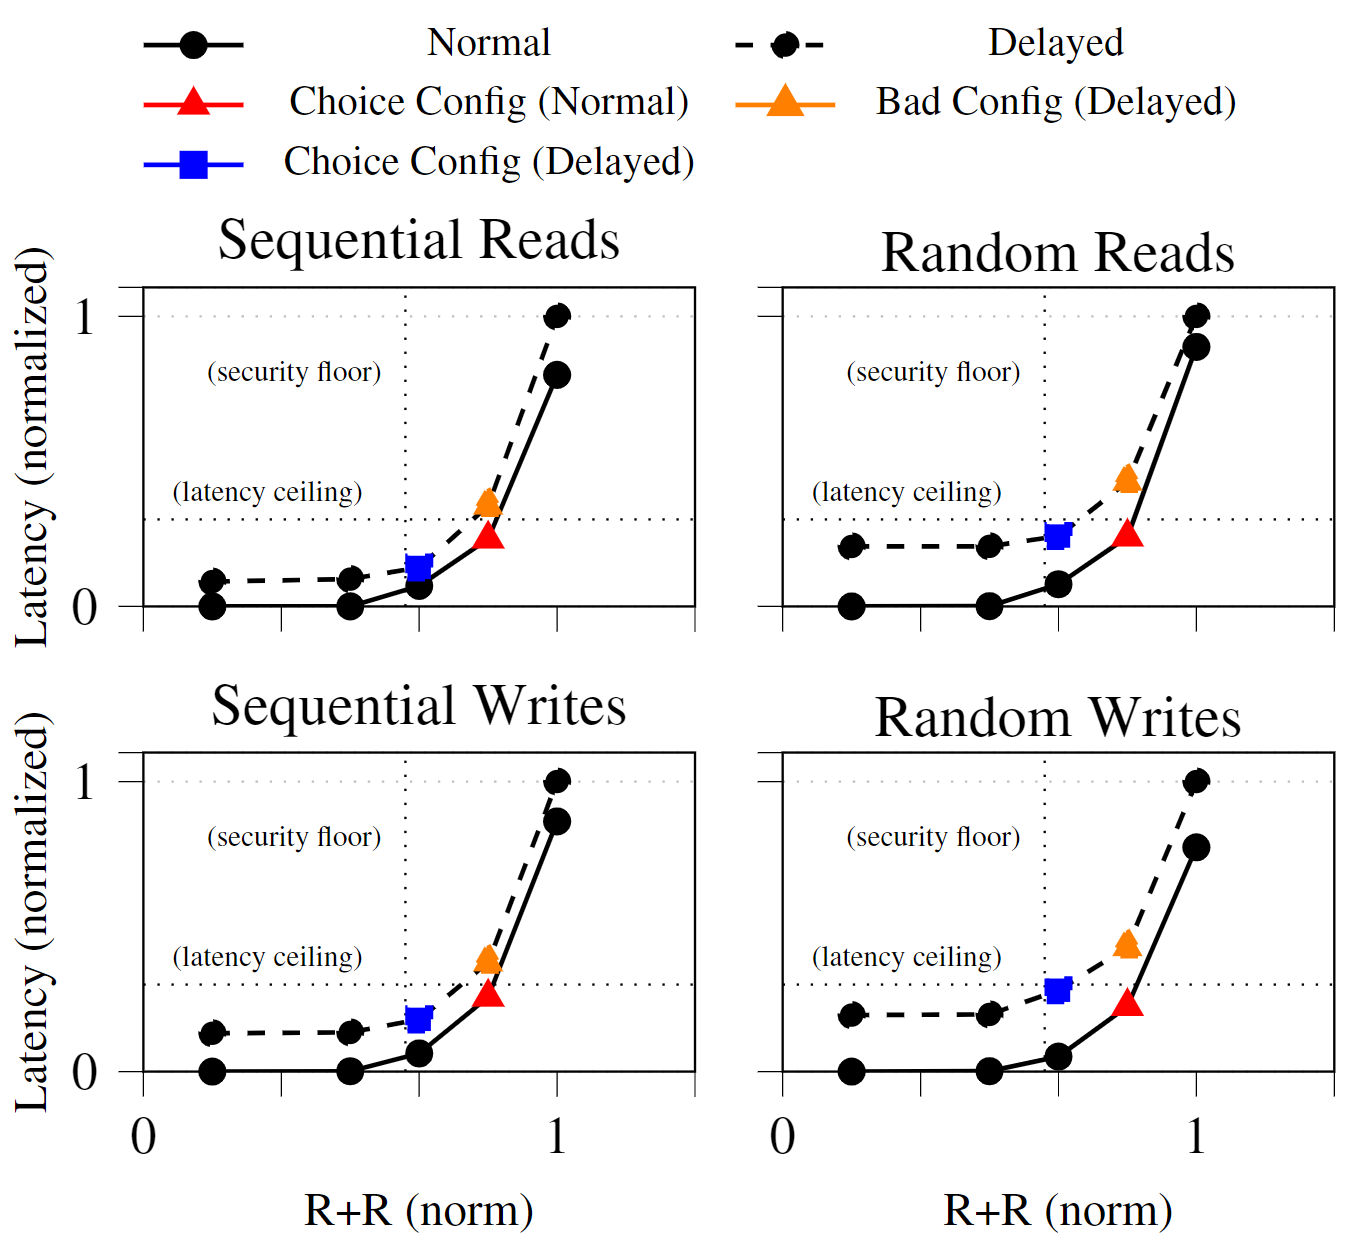
\includegraphics[width=10cm]{figs/sc/screenie.png}}
   \caption{Median sequential and random 40MB read and write performance
   comparison: baseline versus simulated faulty block device.}
  \label{fig:usecase-eol-tradeoff}
\end{figure}

In \figref{usecase-eol-tradeoff}, we see the sequential and random read and
write performance of a 40MB workload when nuggets are encrypted exclusively with
our choice ciphers. While the latency ceiling and security floor have not
changed, we see increased latency in the delayed workloads.

Our goal is to remain under the latency ceiling while remaining above the
security floor. Thanks to Forward switching, accesses to highly trafficked areas
of the drive can remain performant even during drive end-of-life.
